\chapter{Introduction}
\label{Chapter: 1}
\lhead{\bfseries INTRODUCTION}

The field of \gls{av} is rapidly evolving, with significant advancements transforming various industries. As these technologies become more sophisticated, they promise to revolutionize transportation, healthcare, and numerous other sectors by enhancing efficiency and safety. This thesis delves into the structure and contributions of such systems, providing a detailed exploration of their current state, challenges, and future potential.



The contributions detailed in this thesis are instrumental in advancing the state of \gls{av} technology across various fields, including: automotive, drones, and railways. By improving perception systems, learning algorithms, and cybersecurity measures, this research addresses both operational unpredictability and digital security threats, paving the way for safer and more reliable autonomous vehicles. 

\gls{av} stands at the vanguard of technological innovation, spearheading profound transformations across a diverse array of industries. Autonomous systems, which include groundbreaking technologies such as \glspl{UAV}, self-driving cars and \gls{vc} hold the promise of significantly enhancing efficiency, safety, and reliability across numerous applications. These applications span critical sectors, including but not limited to transportation, healthcare, agriculture, and security. This PhD thesis, titled "Advancements in Perception, Learning, and Cooperation for Autonomous Vehicles," delves deeply into the fundamental challenges and pivotal breakthroughs in the development of \gls{av}. It places a particular emphasis on advancing perception systems, refining machine learning algorithms, and developing cooperative control architectures, which collectively underpin the next generation of intelligent, autonomous technologies.

\gls{av} represent a significant leap forward in the evolution of technology. These systems extend beyond traditional automation by incorporating advanced decision-making capabilities that allow them to operate independently, learn from their environments, and adapt to new situations. Unlike automated systems, which operate under pre-defined rules, \gls{av} possess the ability to learn and evolve, making them capable of handling complex tasks without human intervention.

The impact of \gls{av} is profound and far-reaching. In the transportation sector, for instance, self-driving cars and UAVs are poised to revolutionize the way people and goods are transported. These technologies promise to reduce traffic congestion, lower accident rates, and increase fuel efficiency. In healthcare, \gls{av} are being developed to assist in surgeries, deliver medications, and provide remote patient monitoring. In agriculture, UAVs are used for precision farming, monitoring crop health, and managing livestock. In security, \gls{av} are employed for surveillance, border control, and disaster response.





\newpage
\section{Contributions}


Figure\tildeAdd\ref{fig:as_topics} presents the primary fields of my contributions on \gls{av} in this thesis: computer vision, learning, cybersecurity, and cooperation. These interconnected domains are crucial for advancing the capabilities and ensuring the reliability of autonomous technologies.


\begin{figure}[h]
	\centering
	


\tikzset{every picture/.style={line width=0.75pt}} %set default line width to 0.75pt        

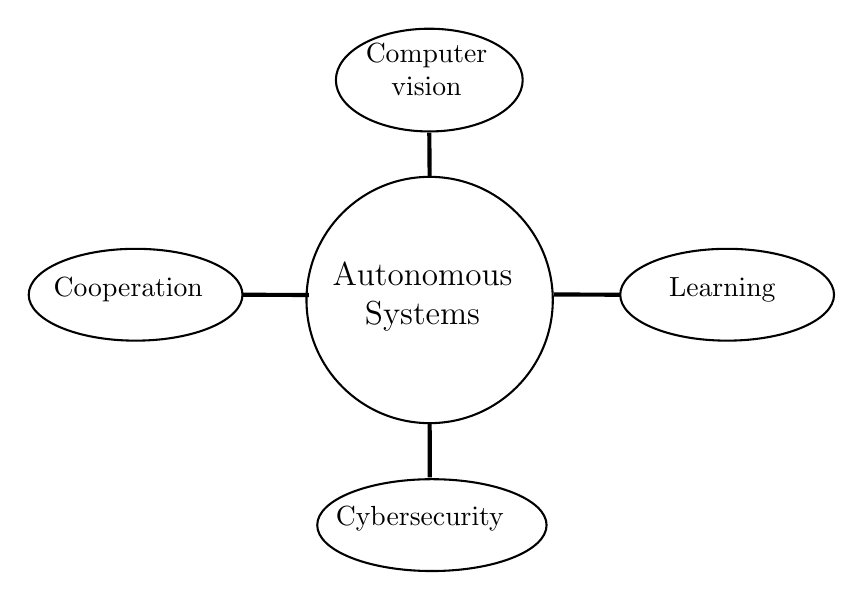
\begin{tikzpicture}[x=0.75pt,y=0.75pt,yscale=-1,xscale=1]
	%uncomment if require: \path (0,300); %set diagram left start at 0, and has height of 300
	
	%Shape: Circle [id:dp5010564721419528] 
	\draw  [fill={rgb, 255:red, 255; green, 255; blue, 255 }  ,fill opacity=1 ] (233.83,138.17) .. controls (233.83,105.4) and (260.4,78.83) .. (293.17,78.83) .. controls (325.94,78.83) and (352.5,105.4) .. (352.5,138.17) .. controls (352.5,170.94) and (325.94,197.5) .. (293.17,197.5) .. controls (260.4,197.5) and (233.83,170.94) .. (233.83,138.17) -- cycle ;
	%Shape: Ellipse [id:dp7493465831132178] 
	\draw  [fill={rgb, 255:red, 255; green, 255; blue, 255 }  ,fill opacity=1 ] (248,32.21) .. controls (248,18.55) and (268.15,7.46) .. (293,7.46) .. controls (317.85,7.46) and (338,18.55) .. (338,32.21) .. controls (338,45.88) and (317.85,56.96) .. (293,56.96) .. controls (268.15,56.96) and (248,45.88) .. (248,32.21) -- cycle ;
	%Shape: Ellipse [id:dp8875049173440994] 
	\draw  [fill={rgb, 255:red, 255; green, 255; blue, 255 }  ,fill opacity=1 ] (100,135.63) .. controls (100,123.41) and (123.06,113.5) .. (151.5,113.5) .. controls (179.94,113.5) and (203,123.41) .. (203,135.63) .. controls (203,147.84) and (179.94,157.75) .. (151.5,157.75) .. controls (123.06,157.75) and (100,147.84) .. (100,135.63) -- cycle ;
	%Shape: Ellipse [id:dp11147192731401834] 
	\draw  [fill={rgb, 255:red, 255; green, 255; blue, 255 }  ,fill opacity=1 ] (239,246.63) .. controls (239,234.41) and (263.74,224.5) .. (294.25,224.5) .. controls (324.76,224.5) and (349.5,234.41) .. (349.5,246.63) .. controls (349.5,258.84) and (324.76,268.75) .. (294.25,268.75) .. controls (263.74,268.75) and (239,258.84) .. (239,246.63) -- cycle ;
	%Shape: Ellipse [id:dp054528874922785464] 
	\draw  [fill={rgb, 255:red, 255; green, 255; blue, 255 }  ,fill opacity=1 ] (385,135.63) .. controls (385,123.41) and (408.06,113.5) .. (436.5,113.5) .. controls (464.94,113.5) and (488,123.41) .. (488,135.63) .. controls (488,147.84) and (464.94,157.75) .. (436.5,157.75) .. controls (408.06,157.75) and (385,147.84) .. (385,135.63) -- cycle ;
	%Straight Lines [id:da3827303466072509] 
	\draw [line width=1.5]    (293,57.57) -- (293.17,78.83) ;
	%Straight Lines [id:da5019108033024944] 
	\draw [line width=1.5]    (203,135.63) -- (235,135.75) ;
	%Straight Lines [id:da534596071783388] 
	\draw [line width=1.5]    (353,135.5) -- (385,135.63) ;
	%Straight Lines [id:da15028090879822753] 
	\draw [line width=1.5]    (293.17,197.5) -- (293.25,223.63) ;
	
	% Text Node
	\draw (238.33,118.83) node [anchor=north west][inner sep=0.75pt]  [font=\large] [align=left] {\begin{minipage}[lt]{74.85pt}\setlength\topsep{0pt}
			\begin{center}
				Autonomous \\Systems
			\end{center}
			
	\end{minipage}};
	% Text Node
	\draw (407,126) node [anchor=north west][inner sep=0.75pt]   [align=left] {Learning};
	% Text Node
	\draw (110.5,126) node [anchor=north west][inner sep=0.75pt]   [align=left] {Cooperation};
	% Text Node
	\draw (246.5,236) node [anchor=north west][inner sep=0.75pt]   [align=left] {Cybersecurity};
	% Text Node
	\draw (258.5,13.21) node [anchor=north west][inner sep=0.75pt]   [align=left] {\begin{minipage}[lt]{47.5pt}\setlength\topsep{0pt}
			\begin{center}
				Computer\\ vision
			\end{center}
			
	\end{minipage}};
	
	
\end{tikzpicture}
	\caption{Relevant topics to the Contributions.}
	\label{fig:as_topics}
\end{figure}

The relentless pursuit of autonomous vehicle technology has reached a pivotal stage where perception systems define the frontier of innovation. Within this purview, the contributions presented in Chapters 3 and 4 of this thesis underscore pivotal enhancements in the perception capabilities of unmanned aerial vehicles (UAVs) and autonomous driving systems, respectively.

Chapter 3 delineates a novel perception algorithm for UAVs, which marries the pure pursuit method with advanced image processing techniques. This hybrid approach leverages the computational simplicity of the pure pursuit method while significantly enhancing the UAV's environmental perception and path tracking ability. The algorithm's distinction lies in its capacity to adapt to varied and complex operational environments—a critical factor for autonomous navigation. By integrating real-time image processing, the algorithm can discern and follow paths with unprecedented accuracy and reduced computational demand. This innovation is not only a testament to the robustness required for autonomous vehicular technology but also aligns with the open-source ethos, enabling wide-scale replication and iterative improvements.

Chapter 4 introduces an Iterative Tree Search (ITS) approach for real-time lane detection, a quintessential task for autonomous driving. The ITS algorithm deviates from traditional lane detection methods that rely on extensive feature extraction and complex models. Instead, it proposes a pixel-level analysis, which streamlines the detection process, rendering it time-efficient and more suited for embedded systems within autonomous vehicles. This method reflects an evolution of perception systems towards greater computational efficiency, enabling the detection process to operate within the stringent temporal constraints of autonomous driving.

The common thread uniting these contributions is their focus on improving perception—a sensory cornerstone for \gls{av}. Perception is not merely about sensing but involves the interpretation of environmental data to make split-second decisions. In autonomous vehicles, the quality of perception directly influences decision-making algorithms, impacting safety, reliability, and the overall user experience.

The significance of these contributions can be viewed through the lens of their practical applicability. The enhanced path tracking algorithm for UAVs is particularly relevant for search and rescue operations, agricultural monitoring, and surveillance—domains where UAVs must navigate autonomously with high precision. Similarly, the ITS algorithm's implications for autonomous driving extend to urban and highway scenarios where reliable lane detection is crucial for maintaining vehicle trajectory and safety.

Furthermore, these advancements contribute to the overarching goal of creating autonomous vehicles that can operate seamlessly alongside human-driven vehicles. By improving perception systems, we edge closer to harmonizing the coexistence of autonomous and manually controlled vehicles, ensuring a safer and more efficient transportation ecosystem.

In conclusion, the thesis presents two pivotal contributions to the field of autonomous vehicle perception. These innovations not only advance the technical capabilities of \gls{av} but also offer insights into the trajectory of future research and development. As the autonomous vehicle industry continues to evolve, the emphasis on perception systems will undoubtedly remain at the forefront, with the potential to redefine transportation as we know it.


This portion of the thesis underscores the advancements in autonomous vehicle (AV) control systems amidst unpredictable scenarios and cybersecurity threats. Chapters 5 and 6 are critical in bolstering the intelligence and safety frameworks that underpin AV technology.

Chapter 5 presents an innovative approach to AV control using Deep Reinforcement Learning (DRL), specifically adopting the Deep Deterministic Policy Gradient (DDPG) method. This method optimizes the AV's ability to navigate complex environments where pedestrian behavior is unpredictable. The DDPG algorithm is a breakthrough, enabling AVs to learn optimal control policies offline, which are crucial for real-time adaptive driving strategies. The algorithm's efficacy is demonstrated through a series of simulations where the AV must balance pedestrian safety with adherence to its driving trajectory. The results indicate a robust performance in terms of learning speed and quality of the driving policy, ensuring the AV's operational safety in pedestrian-rich environments.

Chapter 6 delves into the realm of cybersecurity, introducing a proactive cyber-attack detection and countermeasure strategy, particularly during critical driving maneuvers such as overtaking. It proposes the Intelligent Model Predictive Control System (I-MPS), an architecture that integrates control, prevention, and mitigation mechanisms against cyber threats. The I-MPS utilizes machine learning algorithms to predict and neutralize cyber-attacks in real-time, preserving the integrity of the AV's control systems. This system is pivotal in ensuring that AVs can maintain safety and performance standards, even in the face of sophisticated cyber-attacks. The chapter illustrates the I-MPS's effectiveness through simulations, highlighting its rapid response to threats and its capacity to uphold safe driving practices.

The contributions detailed in these chapters are instrumental in advancing the state of AV technology. The DDPG algorithm's application to pedestrian unpredictability addresses a critical aspect of urban AV deployment, providing a pathway to more nuanced and responsive driving behaviors. Concurrently, the I-MPS framework equips AVs with the necessary defenses against evolving cybersecurity risks, a concern of increasing significance as AVs become more interconnected.

Moreover, these chapters contribute to the broader discourse on AV reliability and trustworthiness. By enhancing learning algorithms and cybersecurity measures, the thesis advocates for a multifaceted approach to AV safety that accommodates both operational unpredictability and digital security threats. These advancements serve as a foundation for future research, potentially influencing regulations and standards for AV deployment.

In essence, the research presented in these sections not only propels technological capabilities but also addresses societal expectations for secure and intelligent AVs. As the AV industry progresses, the insights from this thesis will be vital in shaping the trajectory of AV development, prioritizing resilience, adaptability, and security in an ever-evolving vehicular landscape.










\section{Structure of thesis }

The thesis is divided into three parts, each containing a detailed literature review. These reviews synthesize current research, identify existing knowledge gaps, and set the context for the thesis. They not only provide a backdrop for the subsequent analysis but also highlight the innovative contributions of this research in addressing key issues within the field. \newline

\textbf{Chapter \textcolor{red}{\ref{background}} - Background. \newline} This chapter explores the evolution and impact of autonomous systems, emphasizing their transformative role across various sectors. Autonomous systems form the foundation of \gls{av}, driving their evolution and transformative impact across various sectors. Autonomous systems excel at perceiving, planning, and controlling within complex environments, using multi-source sensors, advanced software, and machine learning algorithms. They make intelligent, autonomous decisions, enhancing efficiency and safety. By spotlighting their architecture, technological breakthroughs, and future trends, this chapter contextualizes how autonomous systems shape the future of automation, revolutionizing transportation, healthcare, and beyond, while addressing societal implications and challenges. \newline \newline
\textbf{Part \textcolor{red}{\ref{part:1}} PERCEPTION} 
\begin{itemize}
	\item \textbf{Chapter \textcolor{red}{\ref{Chapter:1}} - Enhanced Vision-Based UAV Path Following Strategy. \newline }
	Reports  the development of a novel algorithm that synergizes the pure pursuit path tracking methodology with advanced image processing techniques. This integration is specifically tailored to address the computational constraints of micro aerial vehicles (MAVs), enabling them to navigate and complete missions with improved accuracy and efficiency. The theoretical underpinnings of the pure pursuit algorithm are outlined, along with its adaptation to UAV flight dynamics and dynamic path detection through image processing. The mathematical models and simulation frameworks used to analyze the numerical results provide a solid foundation for the subsequent analysis. Practical validation was achieved through participation in the IFAC2020 MathWorks Minidrone competition, benchmarking the algorithm's performance against international standards.
	\item \textbf{Chapter \textcolor{red}{\ref{Chapter:2}} - An Iterative Approach for Real-Time Lane Detection. \newline } 
	Involves introducing an innovative lane detection approach for autonomous driving systems using an Iterative Tree Search (ITS) algorithm. Given the growing need for advanced driver-assistance systems (ADAS) and the evolution of autonomous vehicles, lane detection remains a critical challenge demanding high accuracy and computational efficiency. The ITS algorithm operates directly at the pixel level, bypassing traditional feature extraction methods and complex mathematical modeling. Its lower computational complexity makes it ideal for low-power embedded systems, offering resource-efficient adaptability across various driving conditions. Experimental evaluation in real-world driving scenarios demonstrates the algorithm's robustness in fluctuating illumination and diverse road conditions.
\end{itemize}
\textbf{Part \textcolor{red}{\ref{part:2}} LEARNING} 
\begin{itemize}
	\item \textbf{Chapter \textcolor{red}{\ref{Chapter:3}} - Reinforcement Learning for Collision Avoidance. \newline}
	Focuses on enhancing pedestrian collision avoidance through Deep Reinforcement Learning (DRL) with the Deep Deterministic Policy Gradient (DDPG) algorithm. This integration of DRL in autonomous driving systems marks a paradigm shift towards adaptive, intelligent, and safer navigation strategies that dynamically respond to the unpredictability of urban environments. The DDPG algorithm's continuous state and action space learning capabilities enable autonomous vehicles to make nuanced decisions that significantly reduce collision risks.
	\item \textbf{Chapter \textcolor{red}{\ref{Chapter:4}} - A Machine Learning-Control Approach for Cybersecurity. \newline } 
	Introduces an Informative Model Predictive Scheme (I-MPS) to protect autonomous vehicles from cyber-attacks during overtaking maneuvers. The architecture leverages a Constrained Support Vector Machine classifier informed by Nonlinear Model Predictive Control data to distinguish between normal operation and attack scenarios effectively. This approach is innovative in its adaptability to time-varying or nonlinear dynamics, ensuring safe and reliable operation amidst increasingly sophisticated cyber threats.
\end{itemize}
 \textbf{Part \textcolor{red}{\ref{part:3}} COOPERATION}
\begin{itemize}
	\item \textbf{Chapter \textcolor{red}{\ref{Chapter:5}} - Robust and Safe Control Architectures for Virtual Coupling. \newline }
	The increasing demand for railway transportation has strained high-speed railway lines, requiring innovative solutions like \gls{vc} to enhance capacity and efficiency. \gls{vc} allows trains to operate at reduced headways by dynamically adjusting their spacing using real-time data, improving both capacity and reducing delays. ERTMS Level 3 sets the stage for \gls{vc} by transitioning from fixed-block to dynamic systems. This chapter proposes a robust control architecture to manage \gls{vc} operations, addressing communication delays, packet losses, and uncertainties, with a focus on safety. A simulation tool demonstrates the system's effectiveness in improving railway safety and capacity.

\end{itemize}
\textbf{Appendices}
\begin{itemize}
	\item \textbf{Appendix \textcolor{red}{\ref{app:optimalControl}} - Optimization and Optimal Control. \newline  }
		It explores optimization and optimal control methods, focusing on finding optimal control policies for dynamical systems. It covers problem formulation, including state and control vectors and cost functions, and discusses numerical methods like direct and indirect approaches. Additionally, Model Predictive Control (MPC) is presented as an optimization-based control strategy for dynamic systems.
	
	\item \textbf{Appendix \textcolor{red}{\ref{app:Learning}} -  Learning Algorithms. \newline} 
	This appendix provides an overview of key learning algorithms in autonomous systems, focusing on Support Vector Machines  and Deep Deterministic Policy Gradient. SVMs are supervised learning methods for classification and regression, finding the optimal hyperplane to separate data into two classes by solving an optimization problem. DDPG is a reinforcement learning algorithm within Markov Decision Processes (MDPs) that combines deep learning with reinforcement learning. It uses an actor-critic architecture, where the actor suggests actions and the critic evaluates them, aiming to maximize cumulative rewards. These algorithms enhance classification, decision-making, and overall system efficiency in autonomous applications.
\end{itemize}








\section{Author's Publications}

The following list includes my scientific publications, showcasing the contributions and advancements made during my research:

\begin{itemize}
	\item \cite{terlizzi2021vision} \textbf{Terlizzi, M.}, Silano, G., Russo, L., Aatif, M., Basiri, A., Mariani, V.,  Glielmo, L. (2021, June). \textit{A Vision-Based Algorithm for a Path Following Problem}. In 2021 International Conference on Unmanned Aircraft Systems (ICUAS) (pp. 1630-1635). IEEE.
	\item \cite{terlizzi2021novel} \textbf{Terlizzi, M.}, Russo, L., Picariello, E.,  Glielmo, L. (2021, July).\textit{ A novel algorithm for lane detection based on iterative tree search}. In 2021 IEEE International Workshop on Metrology for Automotive (MetroAutomotive) (pp. 205-209). IEEE.
	\item \cite{russo2021reinforcement} Russo, L., \textbf{Terlizzi, M.}, Tipaldi, M.,  Glielmo, L. (2021, September). \textit{A Reinforcement Learning approach for pedestrian collision avoidance and trajectory tracking in autonomous driving systems.} In 2021 5th International Conference on Control and Fault-Tolerant Systems (SysTol) (pp. 44-49). IEEE.
	\item \cite{terlizzi2021CyberSecurity} \textbf{Terlizzi, M.}, Mariani, V.,  Glielmo, L. (2021, September). \textit{A Model Predictive Scheme for Autonomous Vehicles Cybersecurity.} In 2021 5th International Conference on Control and Fault-Tolerant Systems (SysTol) (pp. 66-71). IEEE.
\end{itemize}
The work presented in Chapter\tildeAdd\ref{Chapter:5} is submitted on IEEE Transactions on Control Systems Technology:
\begin{itemize}
	\item \textbf{Terlizzi, M.}, Liuzza, D.,  Glielmo, L. \textit{A Safe and Robust Control System Architecture for Virtual Coupling.}
\end{itemize}





